\documentclass[border=4pt]{standalone}
% Preámbulo común de las figuras. Cada figura es un documento standalone
% que se compila a SVG con scripts/build_figures.sh
\usepackage[utf8]{inputenc}
\usepackage{amsmath}
\usepackage{tikz}
\usepackage[american, siunitx]{circuitikz}
\usetikzlibrary{arrows.meta,calc,decorations.pathmorphing,patterns}
\tikzset{
  >={Stealth[length=2.2mm]},
  eje/.style={->, thin},
  hilo/.style={thick},
}
% Paleta común: tonos medios legibles sobre fondo claro
\definecolor{azul}{RGB}{31,94,168}
\definecolor{rojo}{RGB}{192,57,43}
\definecolor{verde}{RGB}{39,128,73}
\definecolor{naranja}{RGB}{211,120,30}
\definecolor{morado}{RGB}{125,60,152}

\begin{document}
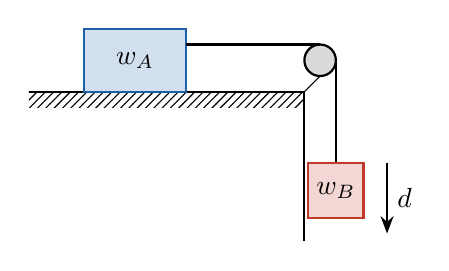
\begin{tikzpicture}[scale=1.0]
  \fill[pattern=north east lines] (-0.5,-0.2) rectangle (3.0,0);
  \draw[thick] (-0.5,0) -- (3.0,0) -- (3.0,-1.9);
  \filldraw[draw=azul, fill=azul!20, thick] (0.2,0) rectangle (1.5,0.8);
  \node at (0.85,0.4) {$w_A$};
  \draw (3.0,0) -- (3.2,0.2);
  \filldraw[fill=gray!30, thick] (3.2,0.4) circle (0.2);
  \draw[hilo] (1.5,0.6) -- (3.2,0.6);
  \draw[hilo] (3.4,0.4) -- (3.4,-0.9);
  \filldraw[draw=rojo, fill=rojo!20, thick] (3.05,-0.9) rectangle (3.75,-1.6);
  \node at (3.4,-1.25) {$w_B$};
  \draw[->, thick] (4.05,-0.9) -- node[right]{$d$} (4.05,-1.8);
\end{tikzpicture}
\end{document}
